% !TEX root = ../main.tex
\label{section:method}

\subsection{Measuring galaxy pitch angle} 
Many methodologies have been proposed and implemented to measure spiral arm properties, including visual inspection (\citealt{2015A&A...582A..86H}), Fourier analysis (i.e. \textsc{2DFFT}, \citealt{2012ApJS..199...33D}), texture analysis (i.e. SpArcFiRe, \citealt{2014ApJ...790...87D}), and combinations of automated methods and human classifiers (\citealt{2017MNRAS.472.2263H}, \citealt{2020MNRAS.493.3854H}). One potentially underused method of obtaining measurements of spirals is through photometric fitting of spiral structure, as possible using tools such as \textsc{GALFIT} \citep{2010AJ....139.2097P} and \textit{Galaxy Builder} \citep{2020arXiv200610450L}. These methods attempt to separate light from an image of a galaxy into distinct subcomponents, such as a galaxy disc, bulge, bar and spiral arms, generally finding the optimum solution using computational optimization. This optimization process, however, is often not robust for complex, many-component models and requires significant supervision to converge to a physically meaningful result \citep{Gao2017:1709.00746v1}. \citet{2020arXiv200610450L} proposed a solution to this problem through the use of citizen science to provide priors on parameters used in computational fitting.

A common assumption when measuring galaxy pitch angle is that observed spiral arms have a constant pitch angle with radius (e.g. \citealt{2012ApJS..199...33D,2013MNRAS.436.1074S,2014ApJ...790...87D}). Spirals of this kind are known as logarithmic spirals and are described by

\begin{equation}
  \label{eq:log-spiral}
r = A\,e^{\theta\tan\phi},
\end{equation}
%
where $\phi$ is the arm's pitch angle, $A$ is an amplitude coefficient and $\theta$ is the polar coordinate. \textbf{Different arms in a galaxy could have different values of $\phi$, however for each arm, $\phi$ is assumed to constant with radius}. One method used to obtain a pitch angle of a galaxy is to fit logarithmic spirals to individually identified arm segments and take the weighted mean of their pitch angles (which often vary by upwards of $10^\circ$, \citealt{2014ApJ...790...87D}). Weighting is determined by the length of the arc segment, with longer being assigned higher weights, i.e. for a galaxy where we have identified $N$ arm segments, each with length $L_i$ and pitch angle $\phi_i$

\begin{equation}
  \phi_\mathrm{gal} = \left(\sum_{i=1}^{N}L_i\right)^{-1}\sum_{i=1}^{N}L_i \phi_i.
\end{equation}

The most commonly used measurement of uncertainty of length-weighted pitch angles is the unweighted sample variance between the arm segments which were identified.

A notable drawback of length-weighted pitch angle is sensitivity to the number and quality of the spiral arm segments; \citet{2017MNRAS.472.2263H} found that only 15\% of the arm segments which were identified using \textsc{SpArcFiRe} \citep{2014ApJ...790...87D} were identified as ``good'' matches to real spiral arms by citizen science classifiers.

Fourier analysis in one- and two-dimensions (as performed by \citealt{2019arXiv190804246D}, \citealt{2012ApJS..199...33D}, \citealt{2018MNRAS.474.2594M}, \textbf{and dating back to the seminal work of \citealt{ConsidereAthanassoula1988}}) is another widely used method of computationally obtaining galaxy pitch angles. Two-dimensional Fourier methods generally decompose a deprojected image of a galaxy into a superposition of logarithmic spirals between inner and outer annuli \citep{2012ApJS..199...33D} and reports the pitch angle with the highest amplitude as the galaxy's pitch angle. \citet{2020MNRAS.493.3854H} combined Fourier analysis of spiral galaxies with a visual tracing of spiral arms, successfully eliminating observed bias in a sample of toy images of galaxies. It is unclear how the variation between pitch angles of individual arms impacts this measurement. \textbf{We note that while this method is able to model non-logarithmic spirals - as a sum of logarithmic spirals with differing pitch angles, most applications of the model favour picking regions of the galaxy in which the pitch angle is constant with radius - e.g. see Section 4.3.2 of \citealt{2012ApJS..199...33D}.}

\subsection{The Galaxy Sample}
The galaxies analysed in this paper are those for which photometric models were obtained in \citet{2020arXiv200610450L}. These are a subset of the \textit{stellar mass-complete sample} in \citet{2017MNRAS.472.2263H}, a sample of low-redshift ($0.02 < z < 0.055$) face-on spiral galaxies selected using data from the NASA-Sloan Atlas \citep{2011AJ....142...31B} and Galaxy Zoo 2 \citep{Willett2013:1308.3496v2}. The \textit{stellar mass-complete sample} ranged in stellar mass from $9.45 < \log(M_* / M_\odot) < 11.05$, with most of the sample between $9.5 < \log(M_* / M_\odot) < 10.0$. A histogram of stellar masses for our subset can be see in Section \ref{section:constraints-on-galaxy-phi}, where variation with stellar mass, to check the impact of this limited mass range, is also investigated. {\bf For the reader's convenience we also reproduce Figure 4 from \citet{2020arXiv200610450L} here (see Figure \ref{fig:stellarmass}) which shows the redshift and stellar mass distribution of our analysis sample compared to the full \textit{stellar mass-complete sample} from \citet{2017MNRAS.472.2263H}. Our choice (see \citet{2020arXiv200610450L} for details) to prefer lower redshift galaxies for {\it Galaxy Builder} analysis is clear in the mass distribution which which results in a sample which favours galaxies $9.5 < \log(M_* / M_\odot) < 10.0$, and includes a smaller number of spirals with masses up to  $\log(M_* / M_\odot) = 11.05$}

\begin{figure*}
  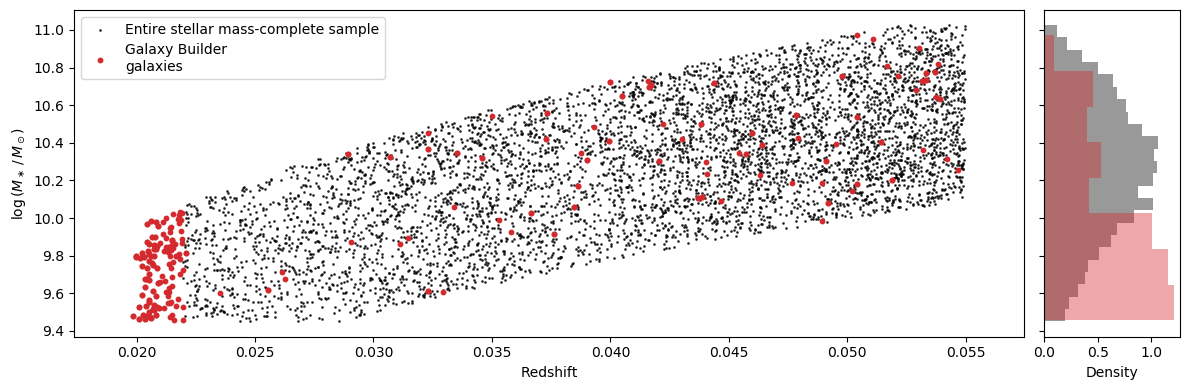
\includegraphics[width=17.7cm]{plots/stellarmass.png}
  \caption{A plot of redshift against stellar mass for the \textit{stellar mass-complete sample} from \citet{2017MNRAS.472.2263H}; the subset we use for analysis in Galaxy Builder are shown in red. At right we show a histogram of the stellar masses. This Figure is identical to Figure 4 from \citet{2020arXiv200610450L} who use the same sample.}
  \label{fig:stellarmass}
\end{figure*}

Some galaxies in \citet{2020arXiv200610450L} were shown to volunteers a second time in a repeat validation subset to create a second aggregate model used to test internal consistency. We combine the 30 classifications of galaxies in this validation subset with the 30 original classifications. Clustering of drawn spiral arms and cleaning of points was then performed as detailed in \citet{2020arXiv200610450L}. We remove any galaxies for which no spiral arms were identified, resulting in a hierarchical data structure of {\bf 129 galaxies, 247 spiral arms and 238,433 points}.

Spiral arm points are deprojected to a face-on orientation using the disk inclination and position angle obtained through photometric model fitting performed in \citet{2020arXiv200610450L}. Arms are individually corrected to all have the same chirality (a pitch angle greater than or equal to zero) using the logarithmic spiral fit in \citet{2020arXiv200610450L}. This was achieved by multiplying the polar coordinate $\theta$ by $-1$ for arms identified as winding counter-clockwise.

\subsection{Bayesian modelling of spiral arms in \textit{Galaxy Builder}}
\label{section:bhsm-model}
In this section, we lay out our Bayesian hierarchical model for galaxy pitch angle. We fit directly to clustered, cleaned points from polylines drawn in \textit{Galaxy Builder}, deprojected and unwrapped to polar coordinates. We fit a logarithmic spiral to each clustered arm (examples are shown in Figure \ref{fig:example-spiral-fits}), with the pitch angles of multiple arms in a single galaxy being drawn from a single parent distribution.

Logarithmic spirals have the desirable properties of a constant pitch angle and a small number of free parameters. \textbf{For this first analysis of the \textit{Galaxy Builder} models we choose to} make use of it here without an explicit comparison to other models. A simple visual inspection of the fitted logarithmic spirals suggests that it is an appropriate model, however, a comparison of a logarithmic spiral profile to other spiral forms (i.e. Archimedian or polynomial) is another important piece of work, outside of the scope of this research, as it has been reported that galaxy arms do not have constant pitch angles (\citealt{1981AJ.....86.1847K}; \citealt{2009MNRAS.397..164R}).

\textbf{As suggested by spiral formation models which correlate a galaxy wide pitch angle, with galaxy wide properties,} we will assume that a give galaxy has some preferred value for arm pitch angle, $\phi_\mathrm{gal}$, and that the pitch angles of spiral arms in that galaxy, $\phi_\mathrm{arm}$, are constant with radius (giving logarithmic spirals) and drawn from a normal distribution centred on $\phi_\mathrm{gal}$, with some spread $\sigma_\mathrm{gal}$ common to all galaxies. We truncate the normal distribution of spiral arm pitch angles in a single galaxy between the physical limits of {0\degree} (a ring) and {90\degree} (a ``spoke''), giving

\begin{equation}
\phi_\mathrm{arm} \sim \mathrm{TruncatedNormal}(\phi_\mathrm{gal}, \sigma_\mathrm{gal}, \mathrm{min}=0, \mathrm{max}=90).
\end{equation}

\textbf{The choice to assume all galaxies show the same inter-arm variation in pitch angle (represented by a common value of $\sigma_\mathrm{gal}$ across all galaxies) was motivated by our small sample size and the low number of arms measured per galaxy. With this sample size we do not find, nor expect to be sensitive to variations in this parameter. It is possible that it does vary between galaxies, and that this variation is physically interesting. Several authors have previously made attempts to measure this parameter.  In a seminal work, \citet{1981AJ.....86.1847K} fit logarithmic spirals to 113 nearby (NGC) galaxies, and note the dominant error in average galaxy pitch angle comes from interarm variation, which they measure to have an average value of 5$^\circ$. \citet{2014ApJ...790...87D} is primarily a machine learning method paper, and while details on the galaxies investigated are not clear, their Table 1 presents the median difference in pitch angle between pairs of arms with different lengths, which varies from 14.5$^\circ$ in very short arms, to 2.6$^\circ$ in the longest traced arms. It is unclear how much this encodes error in their method versus real variation in the galaxy population. Within our own Milky Way, \citet{Vallee2015} did a meta analysis and comparison of several technique to conclude a range of 12-14$^\circ$ was reasonable for all Milky Way spiral arms. In a very detailed study of four very nearby spirals, \citet{HonigRead2015} conclude there are large variations of pitch angles  between spirals, and among arms in a given spiral, but made no comments as to if the variation was consistent with being constant. Further investigation of this issue in a larger \textit{Galaxy Builder} sample would be an interesting follow-up project.}

We assume that the observed points in a \textit{Galaxy Builder} spiral arm, once deprojected, follow a logarithmic spiral with gaussian radial error $\sigma_r$,

\begin{equation}
\widetilde{r_\mathrm{arm}} = \exp\left(\widevec{\theta_\mathrm{arm}}\tan\phi_\mathrm{arm} + c_\mathrm{arm}\right).
\end{equation}

Where $\widetilde{r_\mathrm{arm}}$ is the model's predictions for the radii of the deprojected points in a \textit{Galaxy Builder} arm ($\widevec{r_\mathrm{arm}}$), $c_\mathrm{arm}$ is the amplitude parameter (equivalent to $A$ in Equation \ref{eq:log-spiral}), and $\widevec{\theta_\mathrm{arm}}$ is the polar angles of the points.

We choose hyperpriors over $\phi_\mathrm{gal}$, $\sigma_\mathrm{gal}$, $c_\mathrm{arm}$ and $\sigma_\mathrm{r}$ of

\begin{align}
  \phi_\mathrm{gal} &\sim \mathrm{Uniform}(\mathrm{min}=0, \mathrm{max}=90),\\
  \sigma_\mathrm{gal} &\sim \mathrm{InverseGamma}(\alpha=2,\,\beta=20),\\
  c_\mathrm{arm} &\sim \mathrm{Cauchy}(\alpha=0,\,\beta=10),\\
  \sigma_r &\sim \mathrm{InverseGamma}(\alpha=2, \beta=0.5).
\end{align}

\textbf{These are conservative priors, which are not expected to have significant impact of the results.} The inverse gamma distribution is used to aid the convergence of the Hamiltonian Monte Carlo (HMC) algorithm used (discussed later). The Cauchy distribution is equivalent to the Student's t-distribution with one degree of freedom, and was chosen due to its fatter tails than the normal distribution. Our likelihood function for $N$ arms, each with $n_\mathrm{arm}$ points, is

\begin{equation}
  \mathcal{L} = \prod_{\mathrm{arm}=1}^{N}\left(2\pi\sigma_r^2\right)^{-n_\mathrm{arm}/2}
  \exp\left(-\frac{||\widevec{r_\mathrm{arm}}\,-\,\widetilde{r_\mathrm{arm}}||^2}{2\sigma_r^2}\right).
\end{equation}

We assume that the radial error is Gaussian for simplicity of analysis, however, Shapiro-Wilk tests on the residuals of the logarithmic spirals fit in \citet{2020arXiv200610450L} suggest that this is not a good assumption, and a more robust likelihood (such as the Student's t-distribution) would possibly more appropriate.

To perform inference, we make use of the No-U-Turn-Sampler (NUTS, \citealt{2011arXiv1111.4246H}), implemented in PYMC3\footnote{\url{https://docs.pymc.io/}}, an open-source probabilistic programming framework written in Python \citep{pymc3_paper}. To aid the convergence of MC chains, we scale the radii of deprojected points to have unit variance.
